\documentclass{beamer}
\usetheme{Hannover}
\setbeamersize{sidebar width left=0pt}
\usepackage[T1, T2A]{fontenc}
\usepackage[utf8]{inputenc}
\usepackage[russian]{babel}
\usepackage{hyperref}
\usepackage{graphicx}
\graphicspath{ {../Images/} }

\author{Григорий Матюхин}
\date{\today}
\title{Лабораторная работа \textnumero11.}
\subtitle{Управление загрузкой системы}

\begin{document}
\begin{frame}[plain]
	\titlepage
\end{frame}
\section{Цель работы}
\begin{frame}[plain]
	\frametitle{Цель работы}
	Получить навыки работы с загрузчиком системы GRUB2.
\end{frame}

\subsection{Модификация параметров GRUB2}
\begin{itemize}
	\begin{frame}[plain]
		\frametitle{Модификация параметров GRUB2}
		\item В файле \texttt{/etc/default/grub} удалите параметры \texttt{rhgb} и \texttt{quiet} из строки указания параметров запуска ядра системы:
		\item В этом же файле установите параметр отображения меню загрузки в течение 10 секунд:
		\\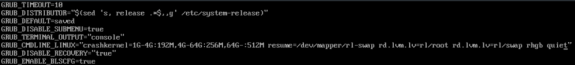
\includegraphics{1.png}
	\end{frame}
	\begin{frame}[plain]
		\item Запишите изменения в GRUB2:
		\\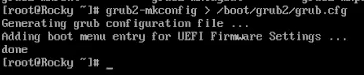
\includegraphics{2.png}
	\end{frame}
\end{itemize}

\subsection{Устранения неполадок}
\begin{itemize}
	\begin{frame}[plain]
		\frametitle{Устранения неполадок}
		\item Запустите (перегрузите) систему. Как только появится меню GRUB, выберите строку с текущей версией ядра в меню и нажмите \texttt{e} для редактирования:
		\item Прокрутите вниз до строки, начинающейся с \texttt{linux (\$root)/vmlinuz-}.
		В конце этой строки введите \texttt{systemd.unit=rescue.target} и удалите опции \texttt{rhgb} и \texttt{quiet} из этой строки, если они там есть:
		\\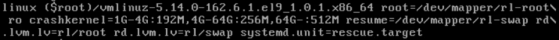
\includegraphics{3.png}
	\end{frame}
	\begin{frame}[plain]
		\item Нажмите \texttt{Ctrl + x} для продолжения процесса загрузки:
		\item Введите пароль пользователя \texttt{root} при появлении запроса:
		\\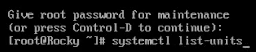
\includegraphics{4.png}
	\end{frame}
	\begin{frame}[plain]
		\item Посмотрите список всех файлов модулей, которые загружены в настоящее время:
		\\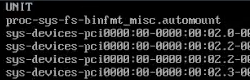
\includegraphics{5.png}
	\end{frame}
	\begin{frame}[plain]
		\item Посмотрите задействованные переменные среды оболочки:
		\\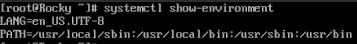
\includegraphics{6.png}
	\end{frame}
	\begin{frame}[plain]
		\item Перегрузите систему.
		\item Как только отобразится меню GRUB, ещё раз нажмите \texttt{e} на строке с текущей версией ядра, чтобы войти в режим редактора. В конце строки, загружающей ядро, введите \texttt{systemd.unit=emergency.target}:
		\\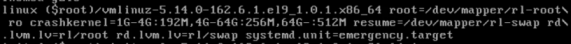
\includegraphics{7.png}
	\end{frame}
	\begin{frame}[plain]
		\item Нажмите \texttt{Ctrl + x} для продолжения процесса загрузки.
		\item Введите пароль пользователя root при появлении запроса:
		\\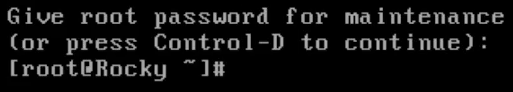
\includegraphics{8.png}
	\end{frame}
	\begin{frame}[plain]
		\item После успешного входа в систему посмотрите список всех загруженных файлов модулей:
		\\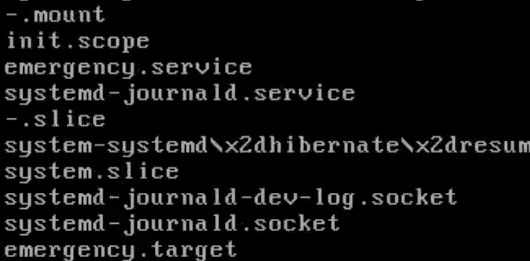
\includegraphics{9.png}
	\end{frame}
\end{itemize}

\subsection{Сброс пароля \texttt{root}}
\begin{itemize}
	\begin{frame}[plain]
		\frametitle{Сброс пароля \texttt{root}}
		\item Запустите (перегрузите) компьютер. Когда отобразится меню GRUB, выберите в меню строку с текущей версией ядра системы и нажмите \texttt{e}, чтобы войти в режим редактора.
		В конце строки, загружающей ядро, введите \texttt{rd.break} и удалите опции \texttt{rhgb} и \texttt{quiet} из этой строки, если они там есть:
		\\
\includegraphics{10.png}
	\end{frame}
	\begin{frame}[plain]
		\item Нажмите \texttt{Ctrl + x} для продолжения процесса загрузки:
		\item Чтобы получить доступ к системному образу для чтения и записи, наберите \texttt{mount -o remount,rw /sysroot}:
		\item Сделайте содержимое каталога \texttt{/sysroot} новым корневым каталогом:
		\\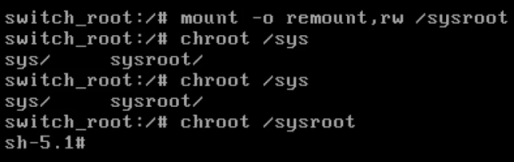
\includegraphics{11.png}
	\end{frame}
	\begin{frame}[plain]
		\item Теперь вы можете ввести команду задания пароля и установить новый пароль для пользователя \texttt{root}:
		\\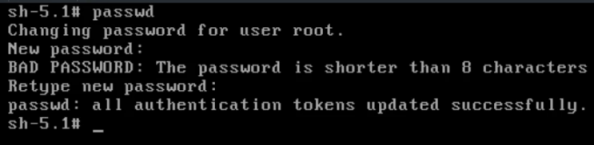
\includegraphics{12.png}
	\end{frame}
	\begin{frame}[plain]
		\item Загрузите политику SELinux:
		\\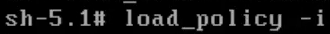
\includegraphics{13.png}
	\end{frame}
	\begin{frame}[plain]
		\item Установите правильный тип контекста для \texttt{/etc/shadow}:
		\\
\includegraphics{14.png}
	\end{frame}
	\begin{frame}[plain]
		\item Перезагрузите систему и войдите в систему с изменённым паролем для пользователя \texttt{root}:
		\\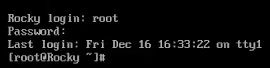
\includegraphics{15.png}
	\end{frame}
\end{itemize}

\section{Вывод}
\begin{frame}[plain]
	\frametitle{Вывод}
	В ходе выполнения данной работы я получил навыки работы с загрузчиком системы GRUB2.
\end{frame}

\end{document}
